\chapter{Background}
%Thorough discovery of background material. Decisions made in the project are correctly informed by background. Analysis of competing products, software standards, necessary software tools, background theory.
% The background section of the report should set the project into context by relating it to existing published work which you read at the start of the project when your approach and methods were being considered. The published work may be in the form of research papers, articles, text books, technical manuals, or even existing software or hardware of which you have had hands-on experience.

\section{Robot's Choice}
There are three robots available for this project: iCub, Baxter and ABB YuMi.

The \citep{iCub} is a 1-metre tall humanoid robot for research in human cognition and artificial intelligence, which has 53 actuated degrees of freedom across its body. Moreover, it has facial expressions and can establish eye contact with users. However, its joints are relatively weaker than Baxter and YuMi. Considering this project only needs vision and robot arms, iCub is not considered as the best robot.

The \citep{baxter} is a two-armed robot which is 3 feet tall and has a pedestal between 5'10" - 6'3" tall. Each of its arms has 7 degrees of freedom, whose movements are more reliable quicker than iCub. Baxter is usually used for simple industry jobs such as unloading, handing of materials. Considering its size, it is not suitable for this project. 

\begin{figure}[H]
\centering
\subfigure[iCub]{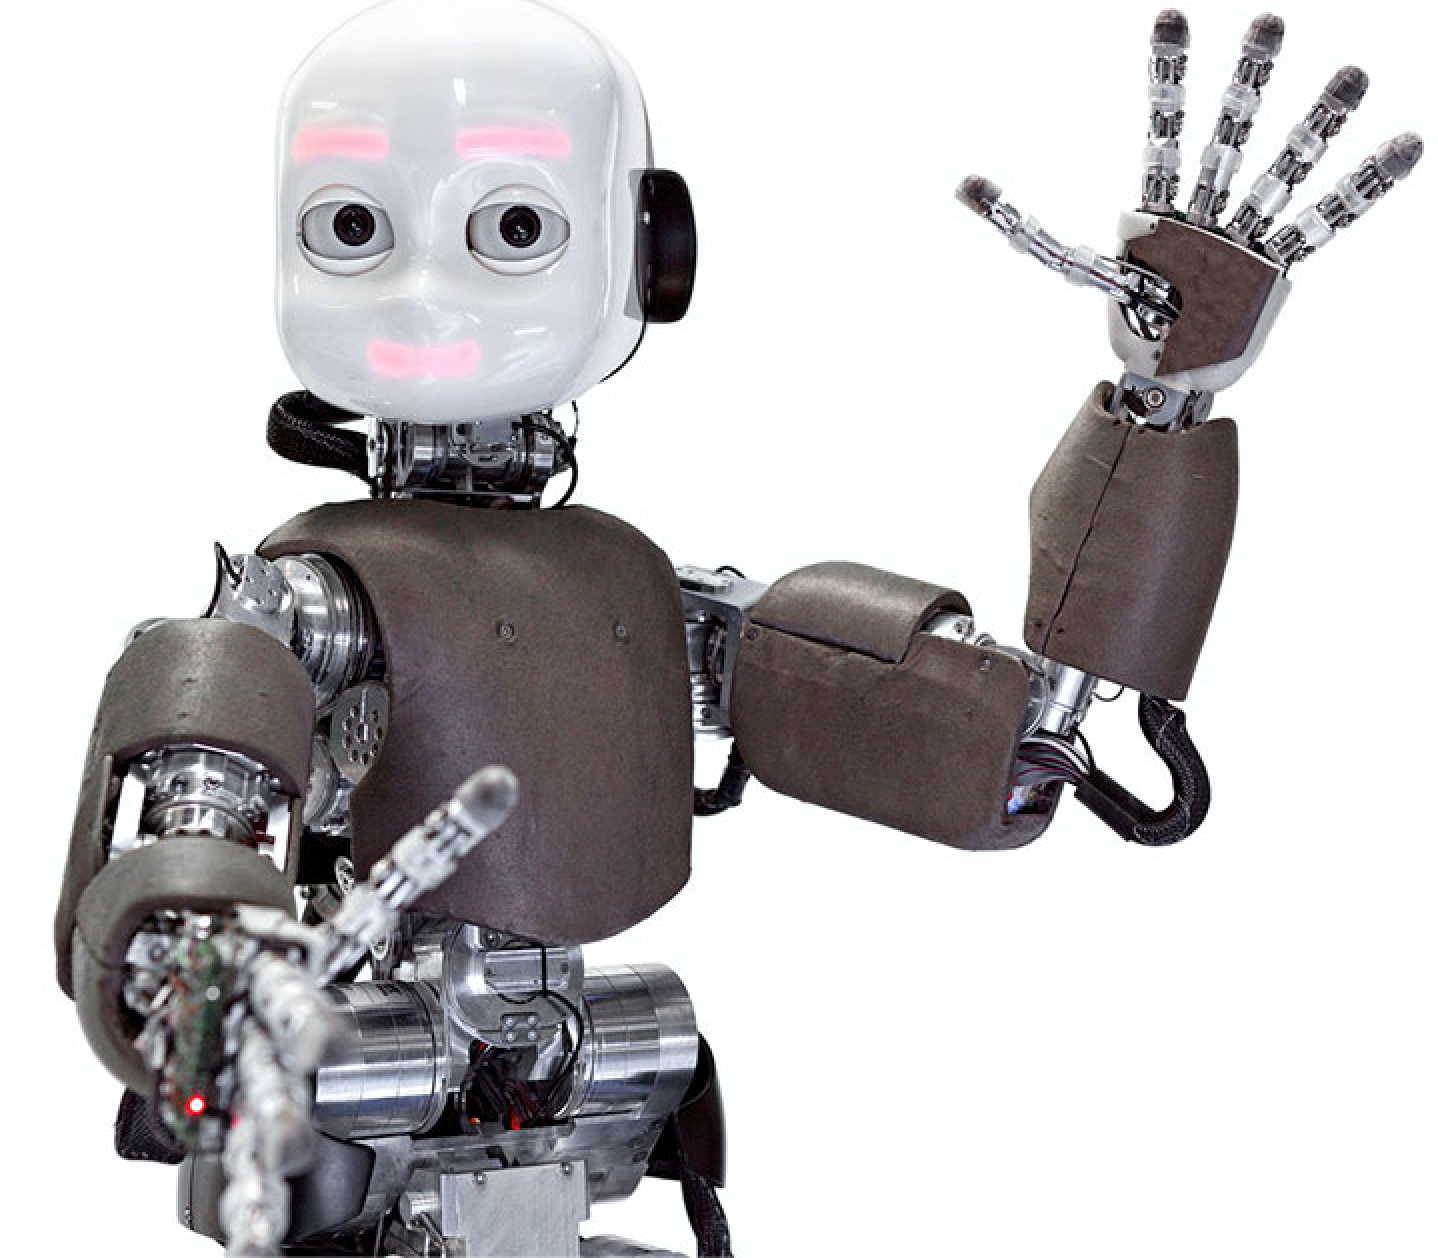
\includegraphics[width = 0.32\columnwidth]{background/icub.png}}
\subfigure[Baxter]{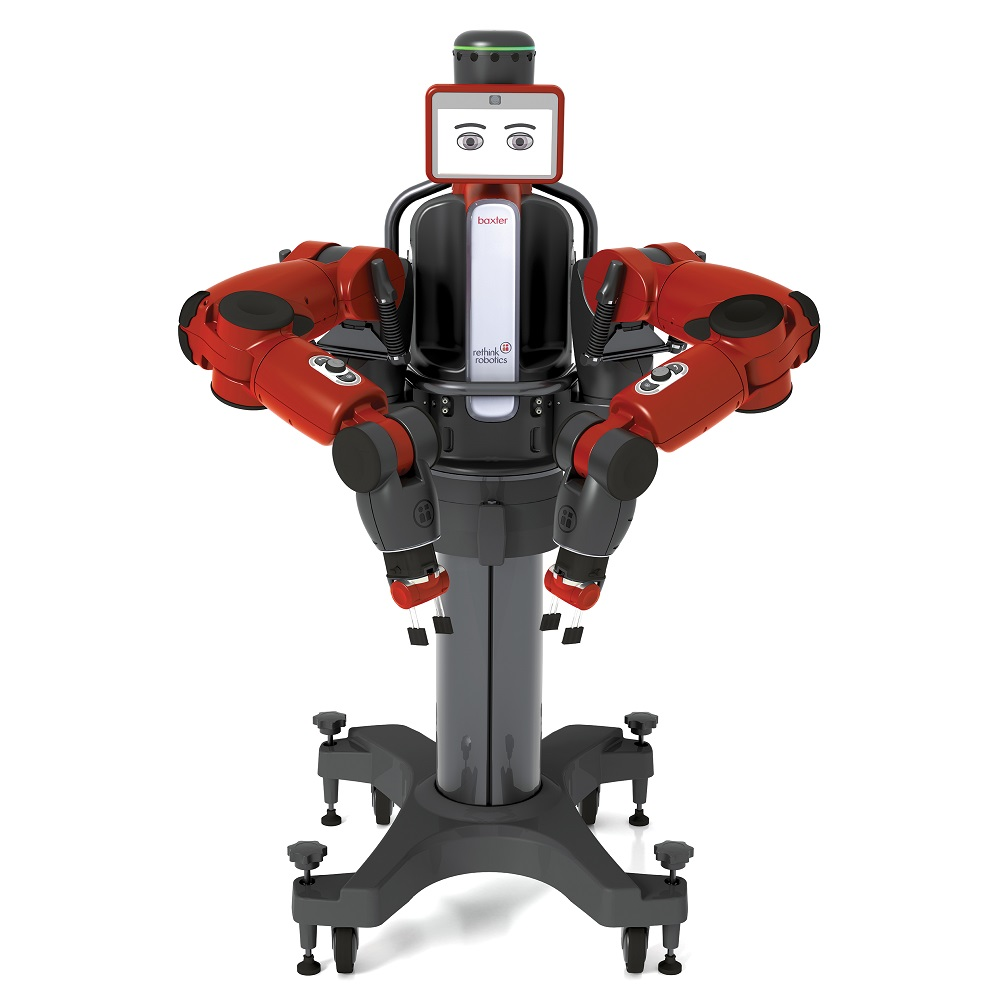
\includegraphics[width = 0.32\columnwidth]{background/baxter.png}}
\subfigure[ABB YuMi]{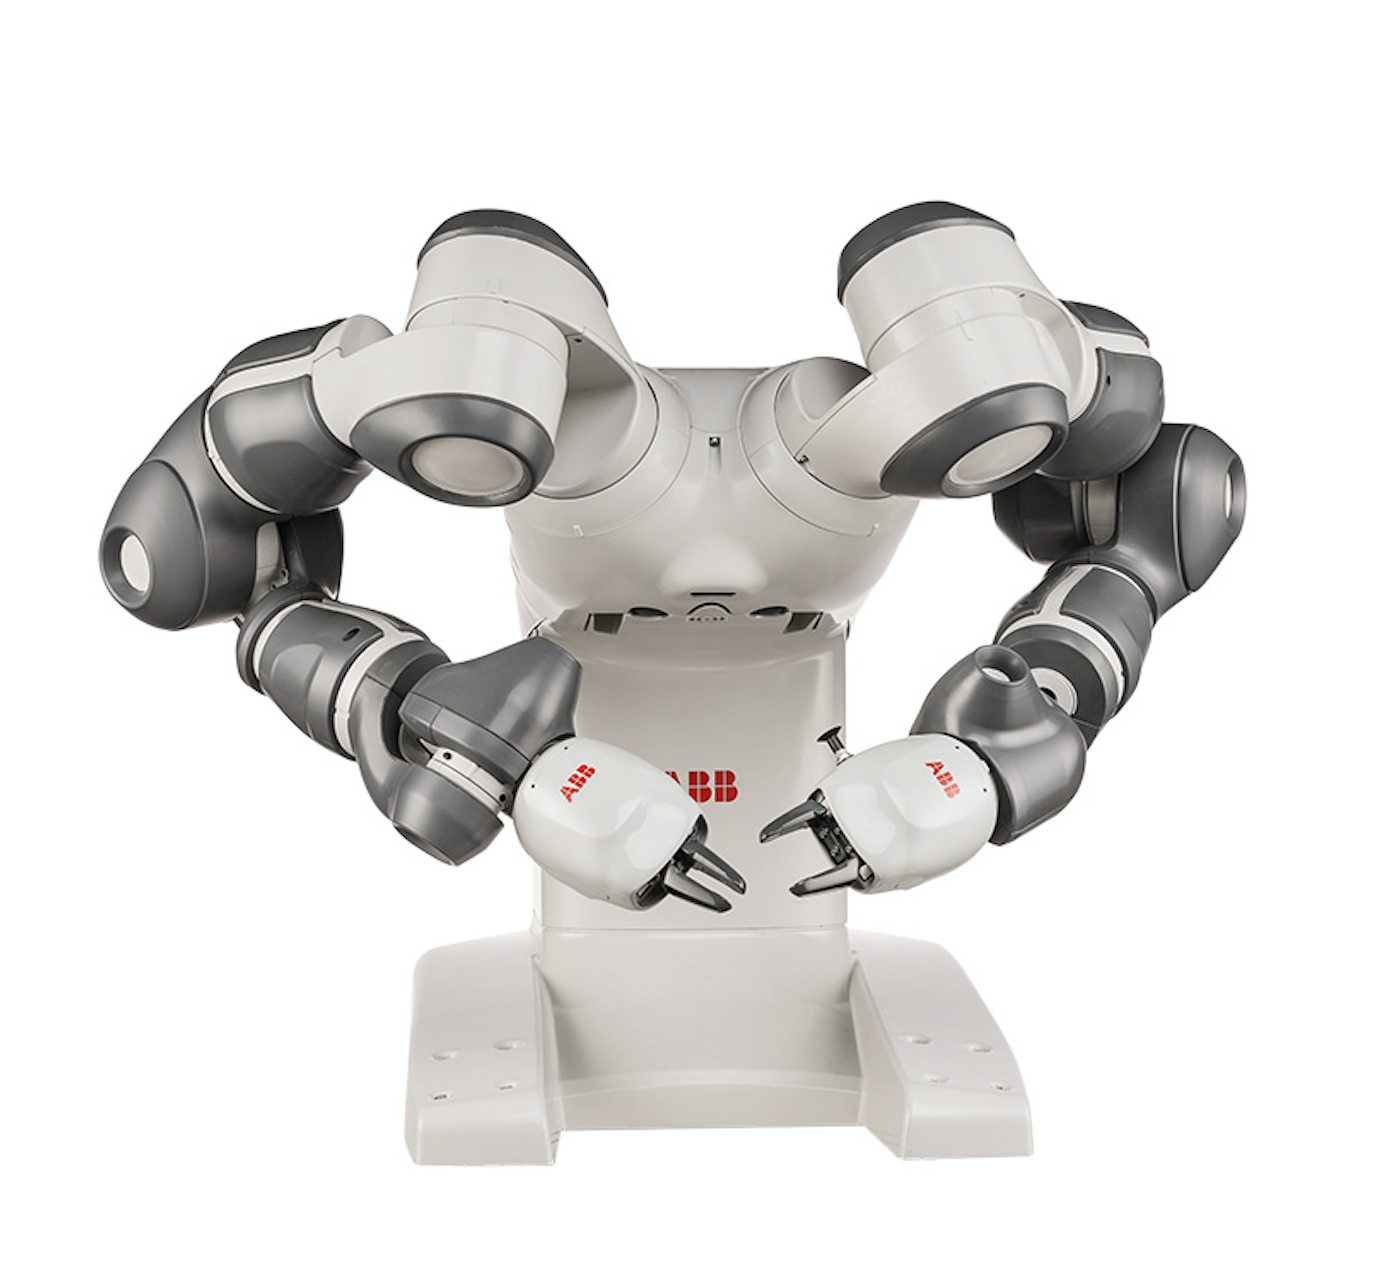
\includegraphics[width = 0.32\columnwidth]{background/YuMi.png}}
\caption{Three available robots}
\label{robot}
\end{figure}

Referring to \citep{ABBsDual5:online}, YuMi is "a collaborative, dual arm, small parts assembly robot that includes flexible hands, parts feeding systems, camera-based part location and state-of-the-art robot control". With 7 degrees of freedom in each arm, it is designed for precise vision-based motion planning and thus is most appropriate to this project.

\section{Motion Planning}
The purpose of robotic motion planning is to seek the solution of the problem of "Go from the start configuration to the goal configuration while respecting all of the robot's constraints", such as avoiding collision with obstacles. A motion planning algorithm takes these tasks description as input, then calculates a path in configuration space. Below are several key concepts in robot motion planning problem.

\begin{itemize}
    \item \textbf{Work Space:} The physical space where the robot operates.
    \item \textbf{Configuration/State Space:} The configuration that describes the robot pose. For a solid 3D robot like YuMi, it can perform both rotation and translation. Therefore, a configuration needs 6 parameters: (x, y, z) for translation and (roll, pitch, yaw) for rotation.
    \item \textbf{Obstacle Space:} The space that robot cannot move to. 
    \item \textbf{Free Space:} The set of configurations of robot that avoids collision with obstacles. In order to test if a configuration is in free space, forward kinematics will firstly be used to calculate the position of robot's geometry, then collision detection will be performed to check if it is collides with environment's geometry.
    \item \textbf{Target Space:} A subspace of free space that consists interested positions we would like the robot to move to. In this project, target space is determined by the camera.
    \item \textbf{Danger Space:} Space that robot is not desired but can move to. The robot usually pass through this space if the trajectory cannot be completed through free space.
\end{itemize}

According to \citep{OMPLPrim20:online}, there are plenty of methods still applicable in many scenarios, including exact and approximate cell decomposition, control-based methods, potential fields, and randomized planning. The summary of each method is as follow.

\begin{itemize}
    \item \textbf{Exact and Approximate Cell Decomposition:} This approach partitions the work space into discrete cells that corresponding to free space, where edges represent adjacency among cells and vertices indicate the individual cells. Therefore, the motion planning problem becomes a search from starting cell to the cell with goal position. This method has a trade off when setting the grid resolution. Coarser grid gives a faster search, but cannot find path for narrow parts of free space. Moreover, the number of points on the grid is exponentially proportional to configuration space dimension, which is inappropriate for this project.
    
    \item \textbf{Control-based Methods:} This method employed control theory and operates in continuous space. It typically uses feedback loops to manipulate the robot with minimal error. However, in complex dynamics environments, it is hard to calculate a feasible trajectory and the valid motions will be restricted.
    
    \item \textbf{Potential Fields:} This technique computes a vector at each point in the work space by summing up the an attractive force emanating from the goal, and a repulsive force from all obstacles. It treats the configuration of robot as a point in a potential field. Although it only requires little computation, navigating using gradient descent to follow the potentials to goal can fail due to local minima in the field.
    
    \item \textbf{Randomized Planning:} Randomization can be effective in motion planning. For example, in potential fields, it has been shown that Brownian motions where applying a random action for a specific amount of time can effectively guide a system out of the local minima.
\end{itemize}

The state-of-art sampling-based motion planning was inspired by randomization \citep{OMPLPrim20:online}, which employs sampling of the configuration space of the robot to effectively answer planning queries. It is especially suitable for systems with many degrees of freedom or differential constraints. Due to motion constraints and size of configuration space, traditional methods can spend a long time to address these problems. While sampling-based planning reasons over a finite set of configurations and connects these samples though collision free paths. Usually, this method gives a probability to complete, as the the number of samples reasoned increases, the probability will converge to 1 if a solution exists. Nevertheless, it cannot determine if a problem has no solution, which can only be speculated by low probability. 

There are many existing sampling-based algorithms, such as Rapidly-expanding Random Trees \citep{RRT}, Probabilistic Roadmap Method \citep{Kavraki1996ProbabilisticRF}, Kinodynamic Planning by Interior-Exterior Cell Exploration \citep{Sucan2012AST} etc. Two typical planners are discussed below.

\begin{figure}[H]
\centering
\subfigure[The 2D work space and a single robot state]{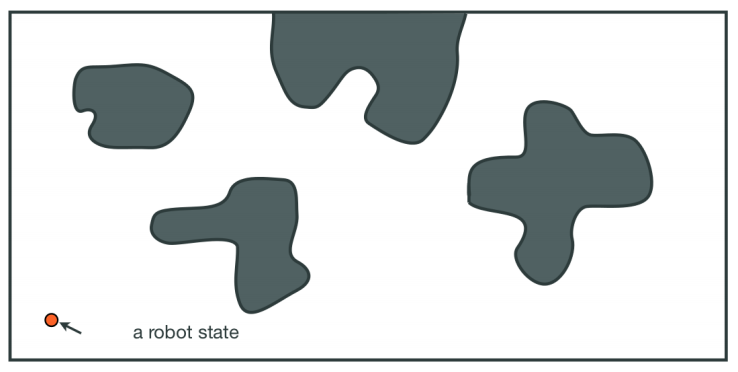
\includegraphics[width = 0.45\columnwidth]{background/rm1.png}}
\subfigure[One possible set of uniform random samples of free space]{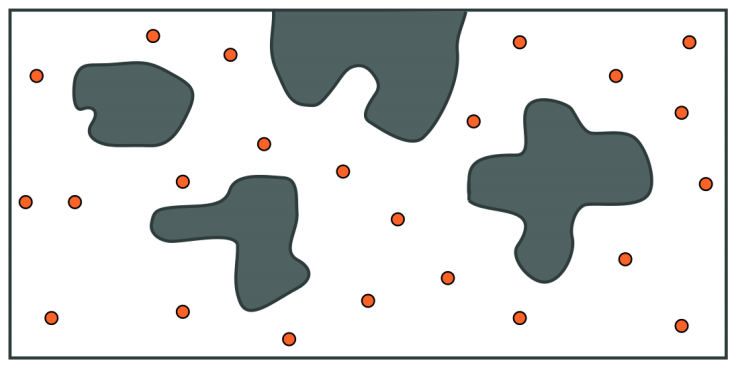
\includegraphics[width = 0.45\columnwidth]{background/rm2.png}}
\subfigure[PRM connects samples that are close to one another using a straight path in the free space]{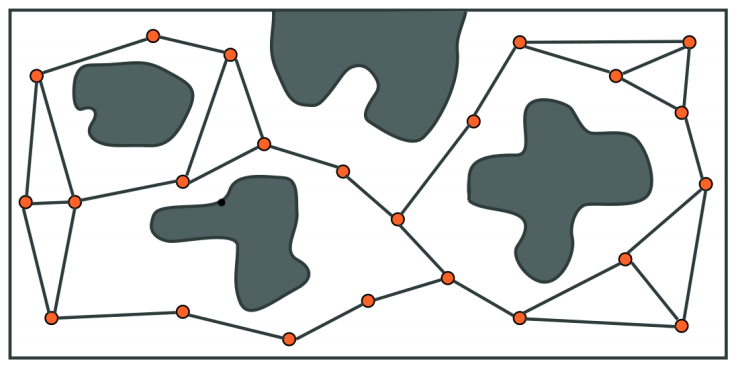
\includegraphics[width = 0.45\columnwidth]{background/rm3.png}}
\subfigure[The start and goal are connected to the roadmap, shortest path is found]{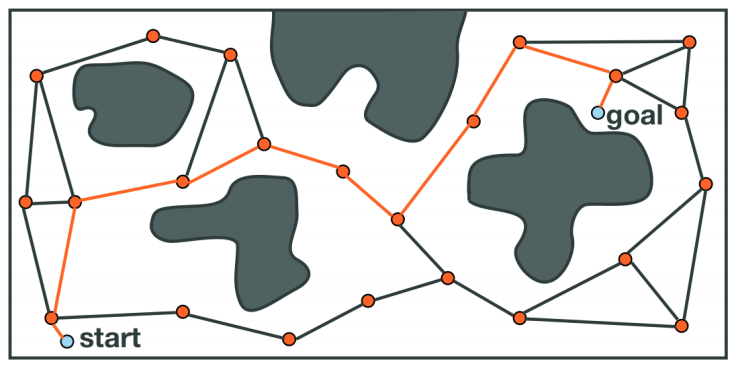
\includegraphics[width = 0.45\columnwidth]{background/rm4.png}}
\caption{Probabilistic roadmap example \citep{OMPLPrim20:online}}
\label{prm}
\end{figure}

\begin{itemize}
    \item \textbf{Probabilistic Roadmap (PRM)} \citep{Kavraki1996ProbabilisticRF}: The idea of this approach is to use random sampling of configuration space to construct a roadmap of free space. Figure \ref{prm} illustrates a simple example of PRM, where a 2D work space and a point robot are used.
    
    The shaded areas represent obstacles. In sampling-based algorithms, free space usually cannot be known. As shown in Figure \ref{prm} (b), after perform collision check, the collision free samples are kept. Once sufficient free samples have been discovered, the roadmap will be built by connecting these samples. Utilizing a local planner whose task is to find short collision free path, each sample will be connected to its k nearest neighbors. Figure \ref{prm} (c) is the complete roadmap for this example. Finally, the start and goal states will be added to the roadmap and a graph search can be fulfilled to compute the shortest path.
    
    \item \textbf{Tree-based Planners:} There are various types of tree-based planners (e.g. \citep{RRT}, \citep{Sucan2012AST}, \citep{inproceedings}, and \citep{hsu}). Here I will describe a general framework, as shown in Figure \ref{tree}. Notice that the biggest difference of tree-based techniques and PRM is that the former structure has no cycles.
    
    Starting from the start state, tree-based planners use random sampling to expansively explore next samples along a collision free path. Figure \ref{tree} (a) illustrates an example of first few valid samples. These planners usually bias their expansion towards the goal, if the existing tree is able to connect to the goal, then they complete the search. Figure \ref{tree} (b) is an example that the goal state cannot be directly connected to the tree, while \ref{tree} (c) shows the case where it can.
    
    Finally, because tree-based planners are directed and acyclic, they are more appropriate for single-query planning and complex dynamics.
\end{itemize}

\begin{figure}[H]
\centering
\subfigure[The first few random valid samples have been connected to the tree using an expansion heuristic]{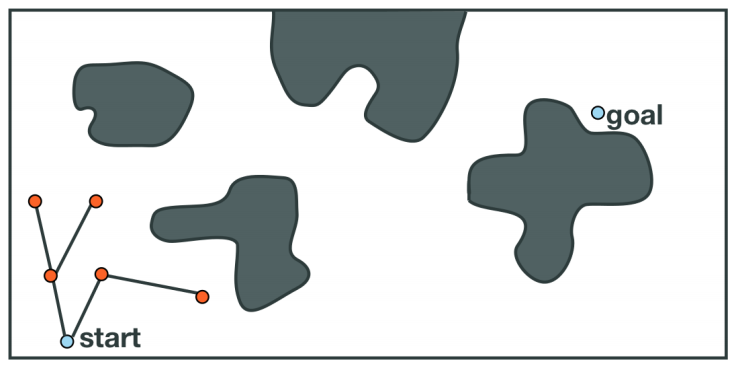
\includegraphics[width = 0.45\columnwidth]{background/rm5.png}}
\subfigure[Case when the goal cannot be connected to the tree because of an obstacle]{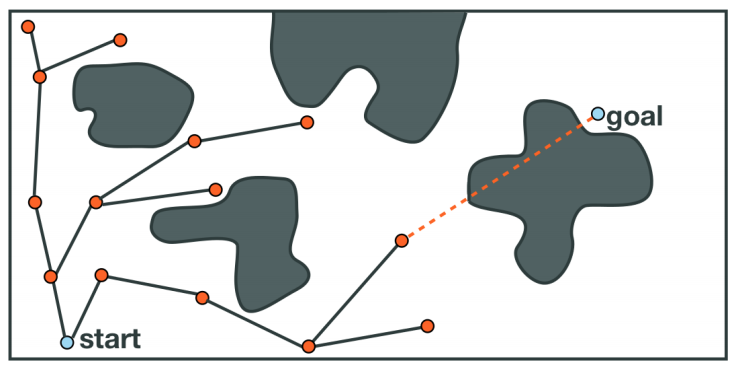
\includegraphics[width = 0.45\columnwidth]{background/rm6.png}}
\subfigure[Case when the goal can be connected to the tree]{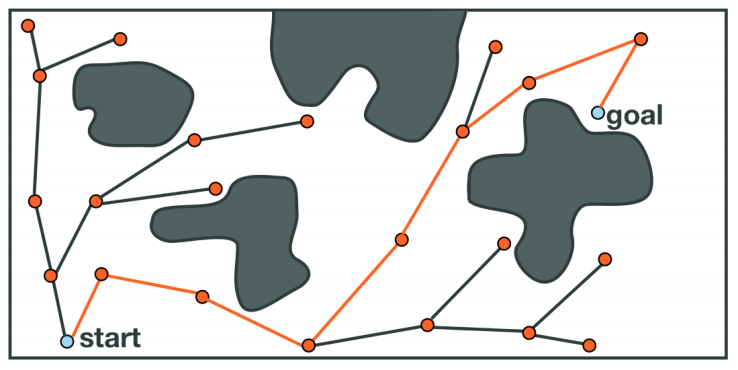
\includegraphics[width = 0.45\columnwidth]{background/rm7.png}}
\caption{Tree-based Planners example \citep{OMPLPrim20:online}}
\label{tree}
\end{figure}

The memory requirement of sampling-based techniques is lower than other types of planners, because no explicit representation of free configuration space is required. It is extremely powerful to plan in complex dynamics and high-dimensional space. However, implementing these algorithms in a generic way is non-trivial. Thus, Open Motion Planning Library (OMPL) \citep{OMPL} is employed to plan the YuMi arm trajectories in this project, which is also available for use through the Robot Operating System (ROS).
In this case, after defining the configuration space, only start state, goal state, and environment scene need to be supplied to plan a single motion. 

\section{Camera's Choice}

Due to the fact that this project requires 3D localization of interested objects (shoes, shoe hole etc.), the camera must be able to provide depth information, which allows user to segment images. There are two types of RGB-D cameras available in the Lab, ASUS Xtion PRO and Microsoft Kinect.

\begin{figure}[H]
\centering
\subfigure[ASUS Xtion PRO]{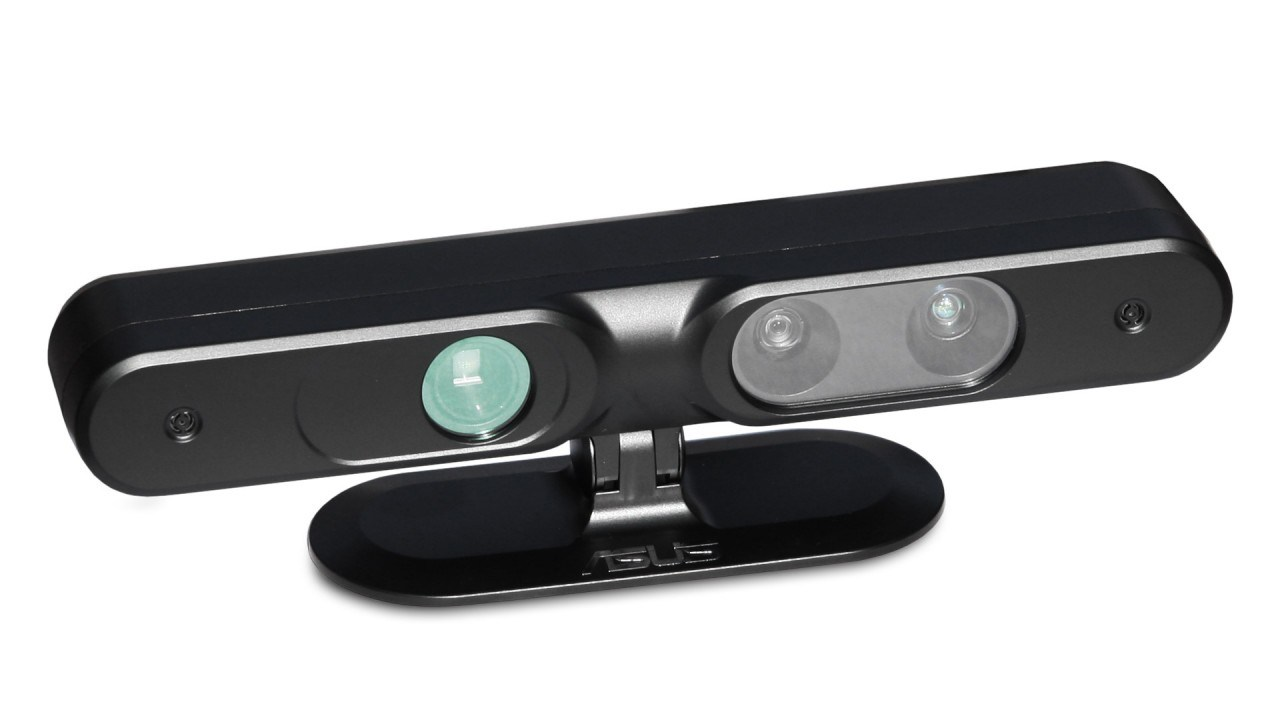
\includegraphics[width = 0.45\columnwidth, height = 40mm]{background/asus.jpg}}
\subfigure[Microsoft Kinect]{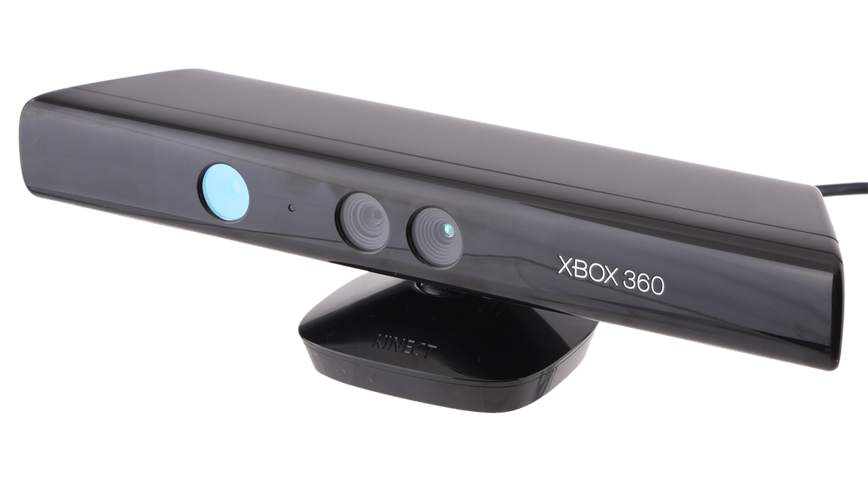
\includegraphics[width = 0.45\columnwidth, height = 36mm]{background/kinect.png}}
\caption{Two available cameras}
\label{camera}
\end{figure}

Both cameras provide similar functionalities, they all have a infrared emitter (leftmost), RGB camera (middle), and a infrared depth camera (rightmost). Considering the ASUS Xtion PRO has already been fixed on the robot, I opted to use it directly for this project.

\section{Object Detection} \label{od}
Object detection is considered as one main part of computer vision, which can provide 2D positions of interested objects from an image. With the help of corresponding depth information provided by ASUS Xtion PRO, 3D location can then be determined. At present, there are several existing methods to detect the object's 2D location.

Due to the fact that the number of occurrences of interested objects is not fixed, and they might have different spatial locations within the image and different aspect ratios, taking different regions from the image and using CNN to classify the presence of the object could computationally blow up \citep{RCNNFast65:online}. Therefore, plenty of detection algorithms like R-CNN \citep{RCNN}, YOLO \citep{YOLO} etc have been developed to tackle this problem. 

The standard R-CNN method is not a complete end-to-end object detector and painfully slow. Fast R-CNN \citep{FastRCNN} improved the detection accuracy and speed, but the model relies on an external region proposal algorithm. With the propose of Faster R-CNN \citep{FasterRCNN}, R-CNNs became an end-to-end object detector which relies on a Region Proposal Network and removes the Selective Search requirement. The advantage of R-CNNs is their accuracy, but the biggest problem of them is their speed, obtaining only 5FPS on a CPU, which is unsuitable for real-time object detection. YOLO employs a one-stage detector strategy to increase the speed of deep learning based object detectors, which obtains 45FPS on a GPU. According to \citep{YOLO9000}, YOLO9000, which trained on both COCO detection dataset and ImageNet classification dataset, is capable of detecting over 9000 separate classes. Although it seems to be suitable for this project, shoelaces and shoe holes are not included in its detection range and its accuracy needs to be tested. YOLOv3 \citep{YOLOv3} is the latest update of YOLO family, however, it is trained only on the COCO dataset that consists 80 labels. The category of shoes is not included, thus it is not suitable for this project. 

Another approach of detecting an object is color detection, which is available for this project. The reason is that shoes with special laces and holes color will be selected as the manipulated object, which should be easily distinguished from background. \citep{cie} converted RGB image to CIE-Lab color space to increase the accuracy of color segmentation. \citep{HSV} performed object segmentation using color filtering based on HSV (Hue, Saturation, Value) and calculated the centroid of the target. Although depth information can help discriminate objects that are not in the same plan as the object of interest, this method still has disadvantage of been sensitive to the changes on lighting and is better being applied on indoor environment. By carefully setting the RBG parameters, this approach will be considered to apply on shoe holes and laces detection.

Shape detection is reckoned as an alternative way, which is achieved by segmenting point clouds and is suitable for detecting shoes. Furthermore, \citep{deformable_track} introduced an algorithm for tracking deformable objects form a sequence of point clouds, which is able to robustly track one-dimensional object such as laces. However, the method is not ready for public consumption right now and following the mathematics steps in the paper to program is quite difficult. 

\citep{vision_touch} presented an object-tracking framework that combines point cloud information from an RGB-D camera with GelSight contact sensor's tactile information. It also improves the pose accuracy during contact and provides robustness to occlusions of small objects. However, it is not suitable for YuMi robot.

Furthermore, OpenPose \citep{openpose} can jointly detect key points of the human body, hand and foot etc with high accuracy and reliability from images, which can also be a backup plan for shoe localization. The only drawback of this approach is that people must wear the shoes in order for the algorithm to locate them, which will increase the complexity of experiments and letting robot manipulate the wearing shoes is considered to be more difficult.

According to these above research, this project will first employ YOLO9000 to detect shoes, and use OpenCV color detection to detect holes and laces. Based on their performances, other approaches will be considered whether to be applied or not.

\section{Orientation Estimation}
In order to manipulate objects using robot, the 3D orientation of interested objects needs to be calculated besides its 3D location (discussed in Section \ref{od}). In this project, particularly, the orientation of shoe holes has to be computed so that the shoe lace can be successfully put into them.

There are several existing 6D object pose estimation (3D location and 3D orientation) methods. \citep{singleshot} proposed a real-time single-shot approach to predict object's 6D pose, which does not require additional post-processing. They first employed CNN to compute 2D image locations of projected vertices of the object’s 3D bounding box. Then a PnP algorithm is utilized to estimated 6D pose. However, these kind of methods become unreliable when low-texture or low-resolution inputs are given. \citep{PoseCNN} introduced PoseCNN, estimates the object's 3D rotation by regressing to a quaternion representation using only color images. They also presented a novel loss function to let PoseCNN handle symmetric objects. Depth data is used for further refinement. \citep{DeepIM} presented DeepIM, given an initial pose estimation, it can refine the object's pose by matching the rendered image against the observed image iteratively. DeepIM only uses color images to introduce the untangled pose representation, which is independent of the 3D object model's coordinate frame and the object size. \citep{DenseFusion} proposed DenseFusion, which processes both color and depth information separately and employs a dense fusion network to extract pixel-wise dense feature embedding, from which the pose of known objects can be predicted. Moreover, it is robust against occlusions and outperforms PoseCNN after refinement on two benchmarks for 6D pose estimation, YCB-Video \citep{PoseCNN} and LineMOD \citep{linemod} respectively.

However, 

Vector xxxxxx 
point cloud library (PCL)

\section{Software}
All programs of this project will run under Ubuntu system. Most programming will use Python, some might be written by C++.

Apart from that, MoveIt! will be used to provide motion planning functionality in ROS, which can load robots' URDF file and create appropriate state spaces for user-defined joint groups and call OMPL planners to find feasible paths. The path produced by OMPL are then translated by MoveIt! into dynamically feasible trajectories. Self-collisions can also be discovered on a pre-processing phase by MoveIt!. 

%A file format for specifying articulated mechanisms is also provided by ROS, when parsed, cause the corresponding state space for planning to be created. 